\documentclass[10pt]{academydoc}
\pagestyle{plain}

% Set Document Details
\doctype{tb} % spec, proc, tb (Specification, Procedure, Technical Bulletin)
\docname{Informative Notes on\\
	SMPTE ST 2065-2 Academy Printing \\*Density (APD) -- Spectral Responsivities, Reference Measurement Device and Spectral Calculation\\* and\\* SMPTE ST 2065-3 Academy Density Exchange Encoding (ADX) -- Encoding Academy Printing Density (APD) Values
}
\altdocname{Informative Notes on SMPTE ST 2065-2 and ST 2065-3}
% Sets the document name used in header - usually an abbreviated document title
\docnumber{TB-2014-005}
\committeename{Academy Color Encoding System (ACES) Project Committee}
\docdate{March 29, 2016}
\summary{
This document provides notes on SMPTE ST 2065-2 Academy Printing Density (APD) -- Spectral Responsivities, Reference Measurement Device and Spectral Calculation and SMPTE ST 2065-3 Academy Density Exchange Encoding (ADX) -- Encoding Academy Printing Density (APD) Values.
}

% Document Starts Here
\begin{document}

\maketitle

% This file contains the content for the Notices
\prelimsectionformat	% Change formatting to that of "Notices" section
\chapter[Notices]{\uppercase{Notices}}
%% Modify below this line %%

\copyright\the\year{} Academy of Motion Picture Arts and Sciences (A.M.P.A.S.). All rights reserved. This document is provided to individuals and organizations for their own internal use, and may be copied or reproduced in its entirety for such use. This document may not be published, distributed, publicly displayed, or transmitted, in whole or in part, without the express written permission of the Academy.

The accuracy, completeness, adequacy, availability or currency of this document is not warranted or guaranteed. Use of information in this document is at your own risk. The Academy expressly disclaims all warranties, including the warranties of merchantability, fitness for a particular purpose and non-infringement.

Copies of this document may be obtained by contacting the Academy at councilinfo@oscars.org.

``Oscars,'' ``Academy Awards,'' and the Oscar statuette are registered trademarks, and the Oscar statuette a copyrighted property, of the Academy of Motion Picture Arts and Sciences.

% This paragraph is optional.  Comment out if you wish to remove it.
This document is distributed to interested parties for review and comment. A.M.P.A.S. reserves the right to change this document without notice, and readers are advised to check with the Council for the latest version of this document.

% This paragraph is optional.  Comment out if you wish to remove it.
The technology described in this document may be the subject of intellectual property rights (including patent, copyright, trademark or similar such rights) of A.M.P.A.S. or others. A.M.P.A.S. declares that it will not enforce any applicable intellectual property rights owned or controlled by it (other than A.M.P.A.S. trademarks) against any person or entity using the intellectual property to comply with this document.

% This paragraph is optional.  Comment out if you wish to remove it.
Attention is drawn to the possibility that some elements of the technology described in this document, or certain applications of the technology may be the subject of intellectual property rights other than those identified above. A.M.P.A.S. shall not be held responsible for identifying any or all such rights. Recipients of this document are invited to submit notification to A.M.P.A.S. of any such intellectual property of which they are aware.

\vspace{10pt}
These notices must be retained in any copies of any part of this document. \newpage
% This file contains the content for the Revision History and 
\prelimsectionformat	% Change formatting to that of "Notices" section
\chapter{Revision History}
%% Modify below this line %%

\begin{tabularx}{\linewidth}{|l|l|X|}
    \hline
    Version & Date       & Description \\ \hline
    1.0     & 12/19/2014 & Initial Version
    \\ \hline
    1.0.1   & 04/24/2015 & Formatting and typo fixes \\ \hline
            & 03/29/2016 & Remove version number - to use modification date as UID \\ \hline
    &   &   \\ \hline
    &   &   \\ \hline
    &   &   \\ \hline
\end{tabularx}

\vspace{0.25in} % <-- DO NOT REMOVE
\chapter{Related Academy Documents} % <-- DO NOT REMOVE
\begin{tabularx}{\linewidth}{|l|X|}
    \hline
    Document Name & Description \\ \hline
    S-2008-001 & Academy Color Encoding Specification (ACES) \\ \hline
    & \\ \hline
    & \\ \hline
    & \\ \hline
    & \\ \hline
\end{tabularx} \newpage

\tableofcontents \newpage

% This file contains the content for the Scope
\cleardoublepage
\numberedformat	
\chapter{Scope} 	% Do not modify section title
%% Modify below this line %%

This document describes the derivation of the ACES white point CIE chromaticity coordinates and details of why the chromaticity coordinates were chosen.  This document includes links to an example Python implementation of the derivation and an iPython notebook intended to help readers reproduce the referenced values.

This document is primarily intended for those interested in understanding the details of the technical specification of ACES and the history of its development. The definition of a color space encoding's white point chromaticity coordinates is one important factor in the definition of a color managed system. The white point used in various ACES encodings does not dictate the creative white point of images created or mastered using the ACES system. It exists to enable accurate conversion to and from the other color encodings such as CIE XYZ.  The proper usage of the ACES white point in conversion, mastering, or reproduction are beyond the scope of this document.  For example, the proper usage of the ACES white point in encoding scene colorimetry in ACES2065-1 is detailed in P-2013-001 \cite{idt}.  

% This section contains the content for the References
\numberedformat
\chapter{References}
The following standards, specifications, articles, presentations, and texts are referenced in this text:
%% Modify below this line %%

SMPTE ST 2065-1:2012, Academy Color Encoding Specification (ACES)

SMPTE RP 177:1993, Derivation of Basic Television Color Equations
% This file contains the content for a main section
\numberedformat
%% Modify below this line %%
\chapter{Notes on SMPTE ST 2065-1}

The document S-2008-001 -- Academy Color Encoding Specification (ACES) was published prior to SMPTE ST 2065-1. S-2008-001 served as the basis for the SMPTE document but is now superseded by the SMPTE standard. S-2008-001, included in Appendix \ref{appendixA} of this document, is provided for historical reference. Those wishing to implement the standard should refer to the SMPTE document, which can be obtained from SMPTE.

\begin{appendices}
	\appendixchapter{Encoding of negative values}{i}
\label{appendixA}

Very small ACES scene referred values below $7\,^1/_4$ stops below 18\% middle gray are encoded as negative ACEScc values. These values should be preserved per the encoding in \autoref{sec:ACEScc} so that all positive ACES values are maintained.

When ACES values are matrixed into the smaller ACEScc color space, colors outside the ACEScc gamut can generate negative values even before the log encoding. If these values are clipped, a conversion back to ACES will not restore the original colors. A specific method of preserving negative values produced by the transformation matrix has not been defined in part to help ease adoption across various color grading systems that have different capabilities and methods for handling negative values. Clipping these values has been found to have minimal visual impact when viewed through the Reference Rendering Transform (RRT) and an appropriate Output Device Transform (ODT) on currently available display technology. However to preserve creative choice in downstream processing and to provide the highest quality archival master, developers implementing ACEScc encoding are encouraged to adopt a method of preserving negative values so that a conversion from ACES to ACEScc and back can be made lossless. Alternatively, a gamut mapping algorithm may be applied to minimize hue shifts resulting from clipping negative ACEScc values. Specific methods for handling negative values may be added to the ACEScc specification in the future.
	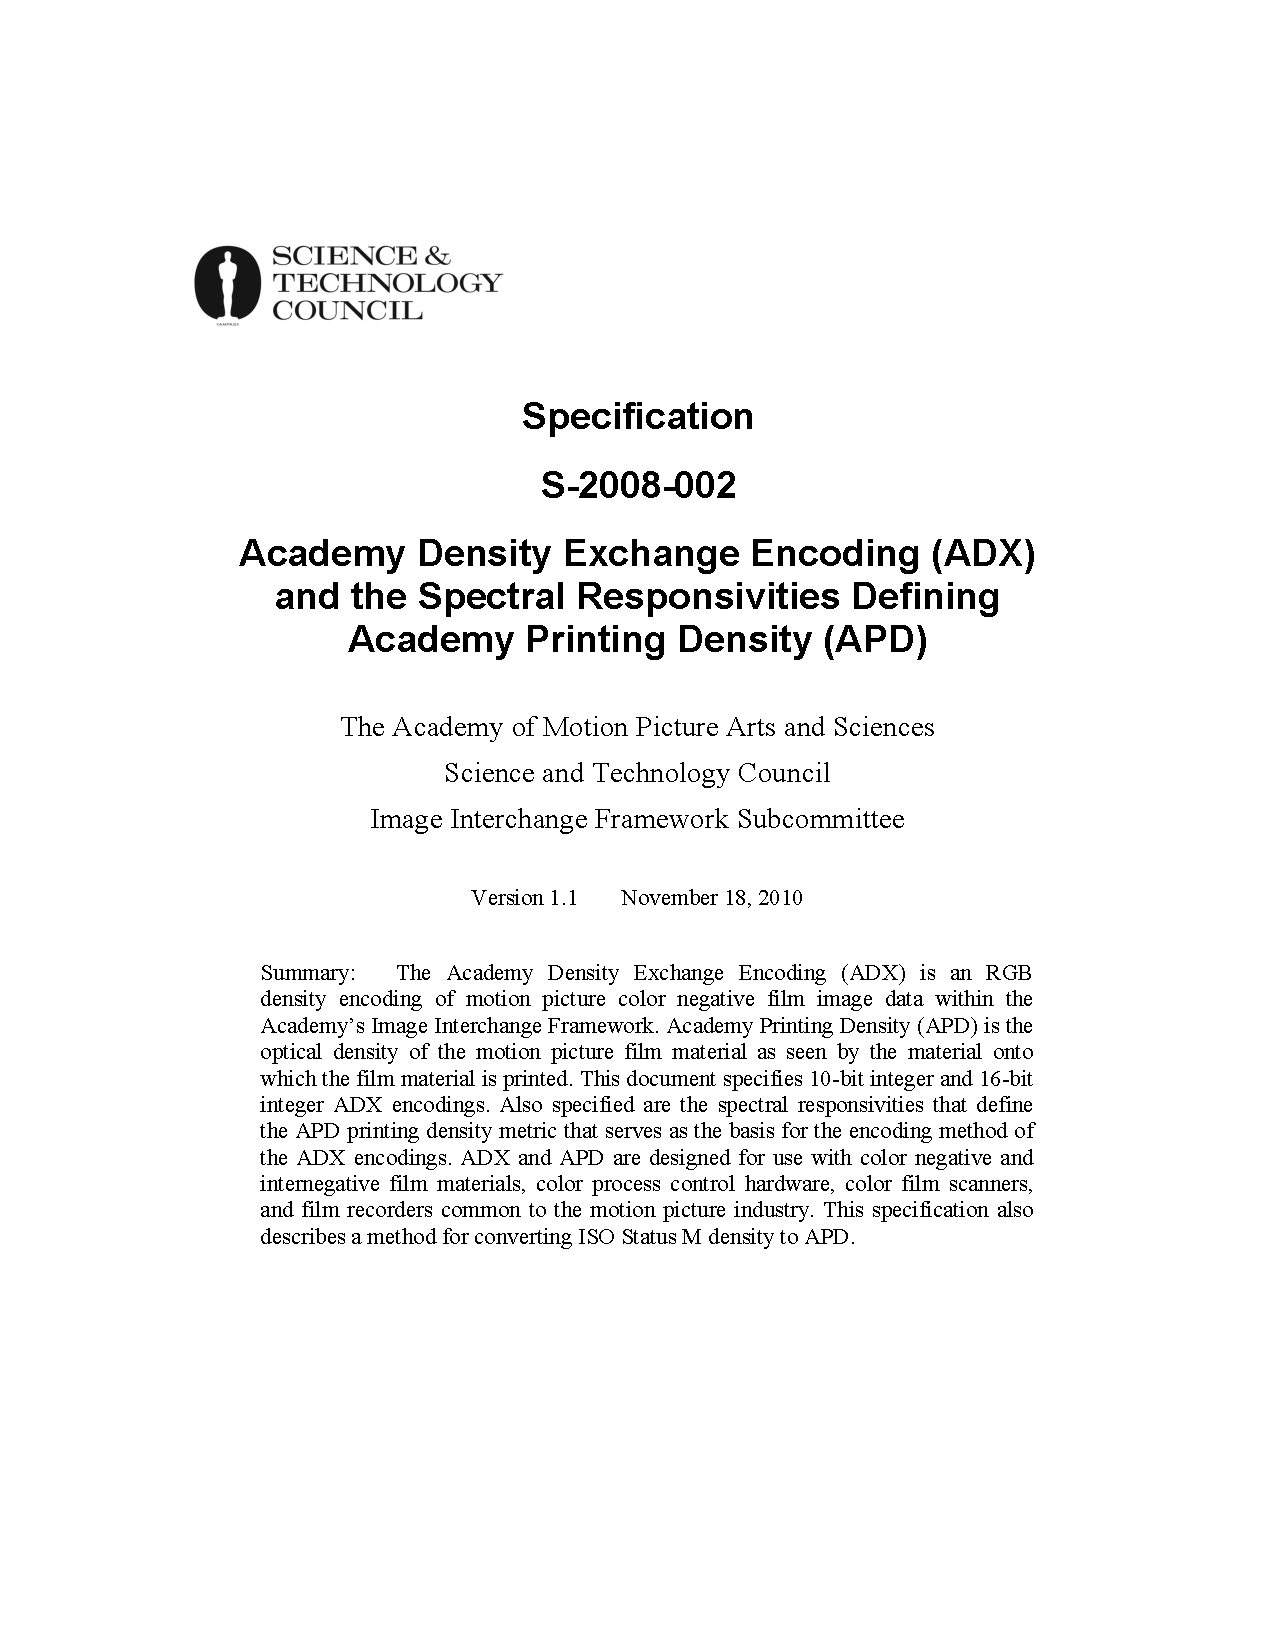
\includepdf[pages={-}]{S-2008-002.pdf}
\end{appendices}

\end{document}